\documentclass[11pt,letterpaper]{article}

% ─── Codificación y lenguaje ────────────────────────────────────────────────
\usepackage[utf8]{inputenc}
\usepackage[T1]{fontenc}
\usepackage[spanish,es-tabla]{babel}
\usepackage{lmodern}
\usepackage{microtype}

% ─── Geometría y formato ────────────────────────────────────────────────────
\usepackage[a4paper,margin=2.5cm]{geometry}
\usepackage{setspace}
\onehalfspacing
\usepackage{parskip}
\usepackage{titlesec}
\titleformat{\section}{\Large\bfseries\sffamily}{\thesection}{0.7em}{}
\titleformat{\subsection}{\large\bfseries\sffamily}{\thesubsection}{0.6em}{}

% ─── Matemáticas ────────────────────────────────────────────────────────────
\usepackage{amsmath, amssymb, amsthm, mathtools}
\usepackage{bm}
\DeclareMathOperator{\diag}{diag}
\DeclareMathOperator{\sgn}{sgn}
\DeclareMathOperator{\tr}{tr}
\DeclareMathOperator{\vecop}{vec}

% ─── Tablas y figuras ───────────────────────────────────────────────────────
\usepackage{booktabs}
\usepackage{multirow}
\usepackage{array}
\usepackage{graphicx}
\usepackage{caption}
\usepackage{subcaption}
\usepackage{float}

% ─── Hipervínculos ──────────────────────────────────────────────────────────
\usepackage{xcolor}
\definecolor{azulItam}{HTML}{1F4E79}
\definecolor{grisCode}{HTML}{F5F5F5}
\definecolor{verdeMatch}{HTML}{2E7D32}
\usepackage[colorlinks=true,linkcolor=azulItam,citecolor=azulItam,urlcolor=azulItam]{hyperref}

% ─── Listings para código MATLAB ────────────────────────────────────────────
\usepackage{listings}
\lstdefinestyle{matlabstyle}{
    backgroundcolor=\color{grisCode},
    basicstyle=\ttfamily\footnotesize,
    keywordstyle=\color{blue!70!black}\bfseries,
    commentstyle=\color{green!50!black}\itshape,
    stringstyle=\color{red!70!black},
    numbers=left,
    numberstyle=\tiny\color{gray},
    numbersep=8pt,
    frame=single,
    rulecolor=\color{gray!40},
    breaklines=true,
    captionpos=b,
    showstringspaces=false,
    language=Matlab,
    morekeywords={fminunc, optimoptions, prctile, randi, chol, qr, randn, fprintf, table, writetable, fullfile, exportgraphics, signs_mp, beta_lower}
}
\lstset{style=matlabstyle}

\lstdefinestyle{rstyle}{
    backgroundcolor=\color{grisCode},
    basicstyle=\ttfamily\footnotesize,
    keywordstyle=\color{blue!70!black}\bfseries,
    commentstyle=\color{green!50!black}\itshape,
    stringstyle=\color{red!70!black},
    numbers=left,
    numberstyle=\tiny\color{gray},
    numbersep=8pt,
    frame=single,
    rulecolor=\color{gray!40},
    breaklines=true,
    captionpos=b,
    showstringspaces=false,
    language=R,
    morekeywords={hpfilter, mutate, ajuste_x13, dplyr, full_join, log}
}

% ─── Algoritmos en pseudocódigo ─────────────────────────────────────────────
\usepackage[ruled,vlined,linesnumbered]{algorithm2e}

% ─── Metadatos ──────────────────────────────────────────────────────────────
\title{
    \vspace{-1.5cm}
    \large\textsc{Instituto Tecnológico Autónomo de México}\\[0.2cm]
    \large Seminario de Investigación\\[0.6cm]
    \Huge\bfseries Replicación de Carrillo \& Elizondo (2018):\\
    \Large Identificación SVAR de choques de política monetaria\\
    en una economía pequeña abierta\\[0.4cm]
    \large \textit{Informe técnico de implementación}
}
\author{Carlos Ramírez \\ \small\texttt{carlos.ramir5285@gmail.com}}
\date{Mayo de 2026}

%==============================================================================
\begin{document}
%==============================================================================

\maketitle

\begin{abstract}
\noindent
Este informe documenta la replicación del ejercicio empírico de Carrillo y Elizondo (2018)\footnote{Carrillo, J.A.\ y Elizondo, R.\ (2018), ``How Robust Are SVARs at Measuring Monetary Policy in Small Open Economies?'', \textit{Journal of Empirical Finance}, 48, 295--314. DOI: \texttt{10.1016/j.jempfin.2018.06.009}.} para México (enero 2001 -- marzo 2014). Se comparan tres estrategias de identificación en un \textsc{svar} bayesiano de seis variables endógenas y tres exógenas \textit{block-exogenous}: restricciones de exclusión recursivas (Cholesky), restricciones de signo estándar (Uhlig, 2005) y restricciones de signo aumentadas con cota de elasticidad de inflación (Kilian y Murphy, 2012). El procesamiento de datos se realizó en \textsf{R} (filtro Hodrick--Prescott, ajuste estacional X-13ARIMA-SEATS, brecha del producto vía filtro de Kalman multifactorial), los diagnósticos en \textsf{Stata} y la estimación estructural en \textsf{MATLAB}. La implementación reproduce los hallazgos centrales del paper: las restricciones de exclusión generan respuestas pequeñas y rezagadas con presencia de \textit{price puzzle}, mientras que las restricciones de signo aumentadas eliminan respuestas implausiblemente grandes de la inflación. La cota de elasticidad estimada por mínimos cuadrados ordinarios con corrección Newey--West (lag = 3) es $\hat\beta_{\text{lower}} = -0{,}721$, comparable al $-0{,}700$ reportado por los autores. Las diferencias residuales se atribuyen a fuentes de datos distintas (Banxico vs.\ \textsc{ifs} en el tipo de cambio real) y al método de ajuste estacional.
\end{abstract}

\vspace{0.3cm}
\noindent\textbf{Palabras clave:} \textsc{svar}, restricciones de signo, política monetaria, descomposición \textsc{qr}, medida de Haar, filtro de Kalman, México.

\vspace{0.6cm}
\hrule
\tableofcontents
\vspace{0.3cm}
\hrule
\vspace{0.6cm}

%==============================================================================
\section{Introducción}
%==============================================================================

La identificación de choques de política monetaria en modelos de vectores autorregresivos estructurales (\textsc{svar}) es uno de los problemas centrales de la econometría macroeconómica aplicada. La clase de identificación elegida determina no solo el signo y magnitud de las funciones impulso--respuesta, sino también la presencia de patrones empíricamente problemáticos como el \textit{price puzzle} —la respuesta positiva de la inflación ante un choque monetario contractivo— o el \textit{exchange rate puzzle} en economías pequeñas.

Carrillo y Elizondo (2018) abordan estas cuestiones en el contexto de México mediante la comparación sistemática de tres estrategias: las restricciones de exclusión recursivas formalizadas por Sims (1980) y adaptadas para economías pequeñas por Cushman y Zha (1997); las restricciones de signo introducidas por Uhlig (2005) y Faust (1998); y una variante aumentada con cota de elasticidad inspirada en Kilian y Murphy (2012). Su contribución metodológica principal es mostrar que la combinación de restricciones de signo con una cota empírica sobre la elasticidad interés--inflación reduce sustancialmente el conjunto de modelos compatibles con las restricciones cualitativas de signo, eliminando aquellos cuyas respuestas serían incoherentes con la magnitud observada en los datos.

Este informe documenta la replicación íntegra de su ejercicio mexicano. La sección~\ref{sec:datos} describe el procesamiento de datos. La sección~\ref{sec:var} especifica el \textsc{var} reducido. Las secciones~\ref{sec:cholesky}, \ref{sec:signos} y \ref{sec:aumentadas} detallan las tres estrategias de identificación con su fundamento matemático e implementación computacional. La sección~\ref{sec:qr} desarrolla, mediante un ejemplo numérico de dimensión $2\times 2$, la lógica de la descomposición \textsc{qr} con corrección de Haar que sustenta el muestreo uniforme de matrices ortogonales. La sección~\ref{sec:beta_lower} discute la estimación de la cota de elasticidad $\hat\beta_{\text{lower}}$, donde el diagnóstico identificó que el método debe ser mínimos cuadrados con corrección Newey--West y no estimación máximo-verosímil con errores \textsc{arma}. La sección~\ref{sec:resultados} compara los resultados con los del paper. La sección~\ref{sec:conclusiones} discute mejoras posibles y conclusiones generales.

%==============================================================================
\section{Datos y procesamiento}\label{sec:datos}
%==============================================================================

\subsection{Fuentes y construcción de variables}

La muestra cubre el periodo enero 2001 -- marzo 2014 a frecuencia mensual, con $T=159$ observaciones, tal y como lo especifica el paper. El bloque doméstico endógeno comprende seis variables expresadas como brechas o tasas de variación, de modo que cumplen estacionariedad bajo las pruebas de raíz unitaria descritas más adelante. El bloque foráneo \textit{block-exogenous} incluye tres variables que capturan la posición cíclica de Estados Unidos y los precios de materias primas. La composición se resume en el cuadro~\ref{tab:variables}.

\begin{table}[H]
\centering
\caption{Variables del modelo y sus fuentes}
\label{tab:variables}
\small
\begin{tabular}{@{}llp{6.2cm}l@{}}
\toprule
\textbf{Símbolo} & \textbf{Nombre} & \textbf{Construcción} & \textbf{Fuente} \\
\midrule
\multicolumn{4}{l}{\textit{Bloque doméstico endógeno}} \\
\midrule
$y$ & \texttt{igae} & Brecha del producto vía filtro de Kalman MFK & Banxico \\
$\pi^c$ & \texttt{pi\_core\_gap} & Inflación subyacente menos tendencia HP & Banxico (SP74625) \\
$\pi^p$ & \texttt{pi\_inpp\_gap} & Inflación al productor menos tendencia HP & Banxico (INPP) \\
$\Delta e$ & \texttt{dep\_tcr} & Variación log del tipo de cambio real ($\times 1200$) & Banxico (SR15997) \\
$i$ & \texttt{i\_gap} & Cetes 28d menos tendencia HP de inflación & Banxico (SF43936) \\
$m$ & \texttt{m2\_gap} & Crecimiento M2 anualizado menos tendencia HP & Banxico (SF12722) \\
\midrule
\multicolumn{4}{l}{\textit{Bloque foráneo block-exogenous}} \\
\midrule
$y^*$ & \texttt{y\_us\_gap} & log(INDPRO) menos tendencia HP & FRED \\
$\pi^*$ & \texttt{pi\_us}    & Inflación PCE anualizada                     & FRED (PCEPI) \\
$\pi^{cm}$ & \texttt{pi\_crb} & Inflación de materias primas anualizada    & CRB Index \\
\bottomrule
\end{tabular}
\end{table}

Conviene resaltar dos elecciones de construcción cuyo efecto se discute más adelante:
la brecha de tasa de interés $i$ se define como la \textit{tasa nominal menos la tendencia HP de la inflación subyacente}, y no como la desviación HP de la propia tasa nominal. Esta elección, congruente con la del paper, convierte $i$ en una aproximación a la tasa real \textit{ex ante} y por tanto en una medida de la postura de política monetaria. Análogamente, la brecha del agregado monetario $m$ resta la tendencia inflacionaria, capturando expansión monetaria real.

\subsection{Ajuste estacional}

Las series de inflación subyacente, inflación al productor y M2 presentan estacionalidad significativa que debe ser removida antes de calcular las brechas. Se utilizó el procedimiento X-13ARIMA-SEATS implementado en el paquete \texttt{seasonal} de \textsf{R}, encapsulado en una función auxiliar que recibe la serie y la fecha de inicio para una correcta asignación de los factores estacionales:

\begin{lstlisting}[style=rstyle, caption={Función de ajuste estacional dinámica (\texttt{0Proc\_data.R})}]
ajuste_x13 <- function(serie_vector, start_date) {
  serie_ts <- ts(serie_vector,
                 start     = c(year(start_date), month(start_date)),
                 frequency = 12)
  ajuste <- seasonal::seas(serie_ts)
  return(as.numeric(seasonal::final(ajuste)))
}
\end{lstlisting}

La fecha de inicio se pasa dinámicamente como \texttt{base\_start <- min(base\$date)} en lugar de fijarse a \texttt{c(2001,1)}, lo cual garantiza la coherencia entre el calendario de la serie original (que comienza en diciembre de 2000) y los factores estacionales estimados. Tras el ajuste, las tasas de variación se calculan en logaritmos y se anualizan multiplicando por 1200, obteniendo así las series base sobre las cuales se aplica el filtro Hodrick--Prescott con $\lambda = 129\,600$ —el valor habitual para datos mensuales sugerido por Ravn y Uhlig (2002)— para extraer la tendencia común $\pi^{\text{trend}}_t$.

\subsection{Brecha del producto vía filtro de Kalman}

A diferencia de las brechas de inflación y dinero, que se obtienen por filtrado HP simple, la brecha del producto se estima mediante un filtro de Kalman \textit{multifactorial} (\textsc{mfk}) sobre el sistema bivariado IGAE--PIB trimestral, siguiendo Elizondo (2012) y la propia recomendación del paper. La rutina \texttt{0b\_brecha\_kalman.R} estima conjuntamente la tendencia y el ciclo en un modelo en espacio de estados que combina la información mensual del IGAE con los puntos de anclaje trimestrales del PIB constante. El resultado se almacena en \texttt{igae\_kalman\_gap.xlsx} y se incorpora al panel final como la columna \texttt{igae}.

La razón para usar el filtro de Kalman en lugar del HP en el producto es que las observaciones trimestrales aportan información sobre el nivel del PIB que no está presente en el IGAE; un HP aplicado solo al IGAE introduciría sesgo de tendencia. El filtro \textsc{mfk} corrige esto al imponer la restricción de igualdad entre las medias trimestrales del IGAE filtrado y los valores del PIB observado.

\subsection{Validación: pruebas de raíz unitaria}

Antes de estimar el \textsc{var} se verificó la estacionariedad de las nueve series mediante las pruebas Augmented Dickey--Fuller (\textsc{adf}) y Phillips--Perron (\textsc{pp}), implementadas en el script \texttt{1DickeyFuller.R}. Las nueve series rechazan la hipótesis nula de raíz unitaria al $5\%$ en al menos una de las dos pruebas, condición suficiente para tratar el sistema como estacionario en niveles (en el caso de las brechas) o en primeras diferencias logarítmicas (en el caso de $\Delta e$, $\pi^*$ y $\pi^{cm}$).

%==============================================================================
\section{Modelo VAR base}\label{sec:var}
%==============================================================================

Sea $\bm{y}_t \in \mathbb{R}^n$ con $n=6$ el vector de variables endógenas y $\bm{z}_t \in \mathbb{R}^{n_z}$ con $n_z=3$ el vector de variables exógenas. El \textsc{var} reducido toma la forma
\begin{equation}
\bm{y}_t = \bm{c} + \sum_{j=1}^{p} \bm{A}_j \, \bm{y}_{t-j} + \bm{C}\,\bm{z}_t + \bm{u}_t,
\qquad
\bm{u}_t \sim \mathcal{N}(\bm{0}, \bm{\Sigma}),
\label{eq:var_reducido}
\end{equation}
donde $p=3$ es el número de rezagos, seleccionado como compromiso entre los criterios de información: \textsc{sic} sugiere uno, \textsc{aic} dos y \textsc{lr} tres. La elección de $p=3$ replica la del paper y deja un balance razonable entre flexibilidad dinámica y eficiencia estadística (con $T=159$ observaciones efectivas y $k=6\cdot 3 + 1 + 3 = 22$ regresores por ecuación, los grados de libertad por ecuación son $T-p-k = 134$).

La estimación se realiza por mínimos cuadrados ordinarios ecuación por ecuación, equivalente al estimador de máxima verosimilitud bajo normalidad. La función \texttt{estimate\_var} en \texttt{SVAR\_SignRestrictions.m} encapsula este procedimiento:

\begin{lstlisting}[style=matlabstyle, caption={Estimación VAR por OLS multivariado}]
function [B, Sigma, resid, X] = estimate_var(Y, Z, p, use_exo)
    [T, n] = size(Y);
    Y_lag = [];
    for lag = 1:p
        Y_lag = [Y_lag, [zeros(lag, n); Y(1:end-lag, :)]];
    end
    Yp = Y(p+1:end, :);
    if use_exo
        Xp = [ones(size(Yp,1),1), Y_lag(p+1:end,:), Z(p+1:end,:)];
    else
        Xp = [ones(size(Yp,1),1), Y_lag(p+1:end,:)];
    end
    B     = (Xp' * Xp) \ (Xp' * Yp);          % k x n  coefs
    resid = Yp - Xp * B;                        % T-p x n residuos
    Sigma = (resid' * resid) / (size(resid,1) - size(Xp,2));
end
\end{lstlisting}

La estabilidad del sistema se verifica calculando los valores propios del polinomio característico $\det(\bm{I}_n - \bm{A}_1 z - \cdots - \bm{A}_p z^p) = 0$. Todos los valores propios reales caen dentro del círculo unitario, garantizando la existencia de la representación \textsc{ma} infinita necesaria para definir las funciones impulso--respuesta.

%==============================================================================
\section{Estrategia 1: Restricciones de exclusión (Cholesky)}\label{sec:cholesky}
%==============================================================================

\subsection{Marco teórico}

La identificación recursiva descansa sobre una ordenación causal de las variables. Dada la matriz de covarianza $\bm{\Sigma}$ de los residuos reducidos, su descomposición de Cholesky $\bm{\Sigma} = \bm{P}\bm{P}'$ (con $\bm{P}$ triangular inferior) define las cargas de impacto $\bm{A}_0 = \bm{P}$ de los choques estructurales sobre las variables. La columna $j$-ésima de $\bm{P}$ es la respuesta de impacto al $j$-ésimo choque estructural; la triangularidad implica que el choque $j$ no afecta contemporáneamente a las variables $1, \ldots, j-1$, sino solo a las variables $j, j+1, \ldots, n$.

El ordenamiento adoptado, lento $\to$ rápido, replica el del paper:
\begin{equation}
y \to \pi^c \to \pi^p \to \Delta e \to i \to m,
\label{eq:orden_chol}
\end{equation}
con la tasa nominal $i$ en la quinta posición, lo cual define el choque de política monetaria como aquel que no afecta de manera contemporánea al producto, a la inflación subyacente, a la inflación al productor ni al tipo de cambio real, pero sí (potencialmente) al agregado monetario M2. Este ordenamiento corresponde al supuesto estándar de política monetaria: el banco central observa las variables reales y de precios al tomar su decisión, mientras que las cantidades de dinero responden endógenamente a la tasa de interés. La columna 5 de $\bm{P}$ es entonces el vector de impacto del choque monetario.

\subsection{Bandas de incertidumbre vía bootstrap}

Para construir las bandas de incertidumbre se implementó el bootstrap recursivo de Runkle (1987), que captura tanto la incertidumbre paramétrica del \textsc{var} como la del esquema de identificación. El procedimiento consiste en re-muestrear los residuos $\bm{u}_t$ con reemplazo, generar pseudo-datos $\bm{y}^{(b)}_t$ por recursión a partir de las condiciones iniciales y los coeficientes estimados, y re-estimar el \textsc{var} en cada réplica. La función \texttt{runkle\_bootstrap\_data} encapsula la generación de la pseudo-muestra:

\begin{lstlisting}[style=matlabstyle, caption={Generación de pseudo-datos por recursión}]
function Y_boot = runkle_bootstrap_data(B, Y, Z, p, res_boot, use_exo)
    [T, n] = size(Y);
    Y_boot = Y;   % primeras p filas = condiciones iniciales
    for t = p+1:T
        y_lags = [];
        for lag = 1:p
            y_lags = [y_lags, Y_boot(t-lag, :)];
        end
        if use_exo
            x_t = [1, y_lags, Z(t,:)];
        else
            x_t = [1, y_lags];
        end
        Y_boot(t, :) = x_t * B + res_boot(t-p, :);
    end
end
\end{lstlisting}

Sobre cada pseudo-muestra se re-estima el \textsc{var}, se aplica Cholesky a la nueva $\bm{\Sigma}^{(b)}$ y se computa la respuesta impulso completa hasta horizonte $h=16$ meses. Con 2\,000 réplicas se construyen las bandas al $68\%$ por percentiles, criterio que también utiliza el paper. La elección del $68\%$ en lugar del $95\%$ tradicional refleja la práctica habitual en \textsc{svar} bayesianos: bandas más estrechas son más informativas sobre la respuesta puntual y menos susceptibles a los problemas de identificación débil que afectan a los intervalos extremos.

\subsection{Resultados Cholesky}

Las funciones impulso--respuesta a un choque monetario contractivo de magnitud unitaria se muestran en la figura~\ref{fig:fig7}. Replican cualitativamente las del paper: la respuesta del producto es prácticamente nula al impacto y crece negativamente con el tiempo; la inflación subyacente exhibe \textit{price puzzle} en los primeros meses (respuesta positiva) que se desvanece tras el sexto mes; el tipo de cambio real se aprecia y luego se deprecia; M2 cae en línea con la teoría. La inclusión de las variables foráneas \textit{block-exogenous} (azul) reduce el price puzzle pero no lo elimina, observación consistente con el hallazgo central del paper.

\begin{figure}[H]
\centering
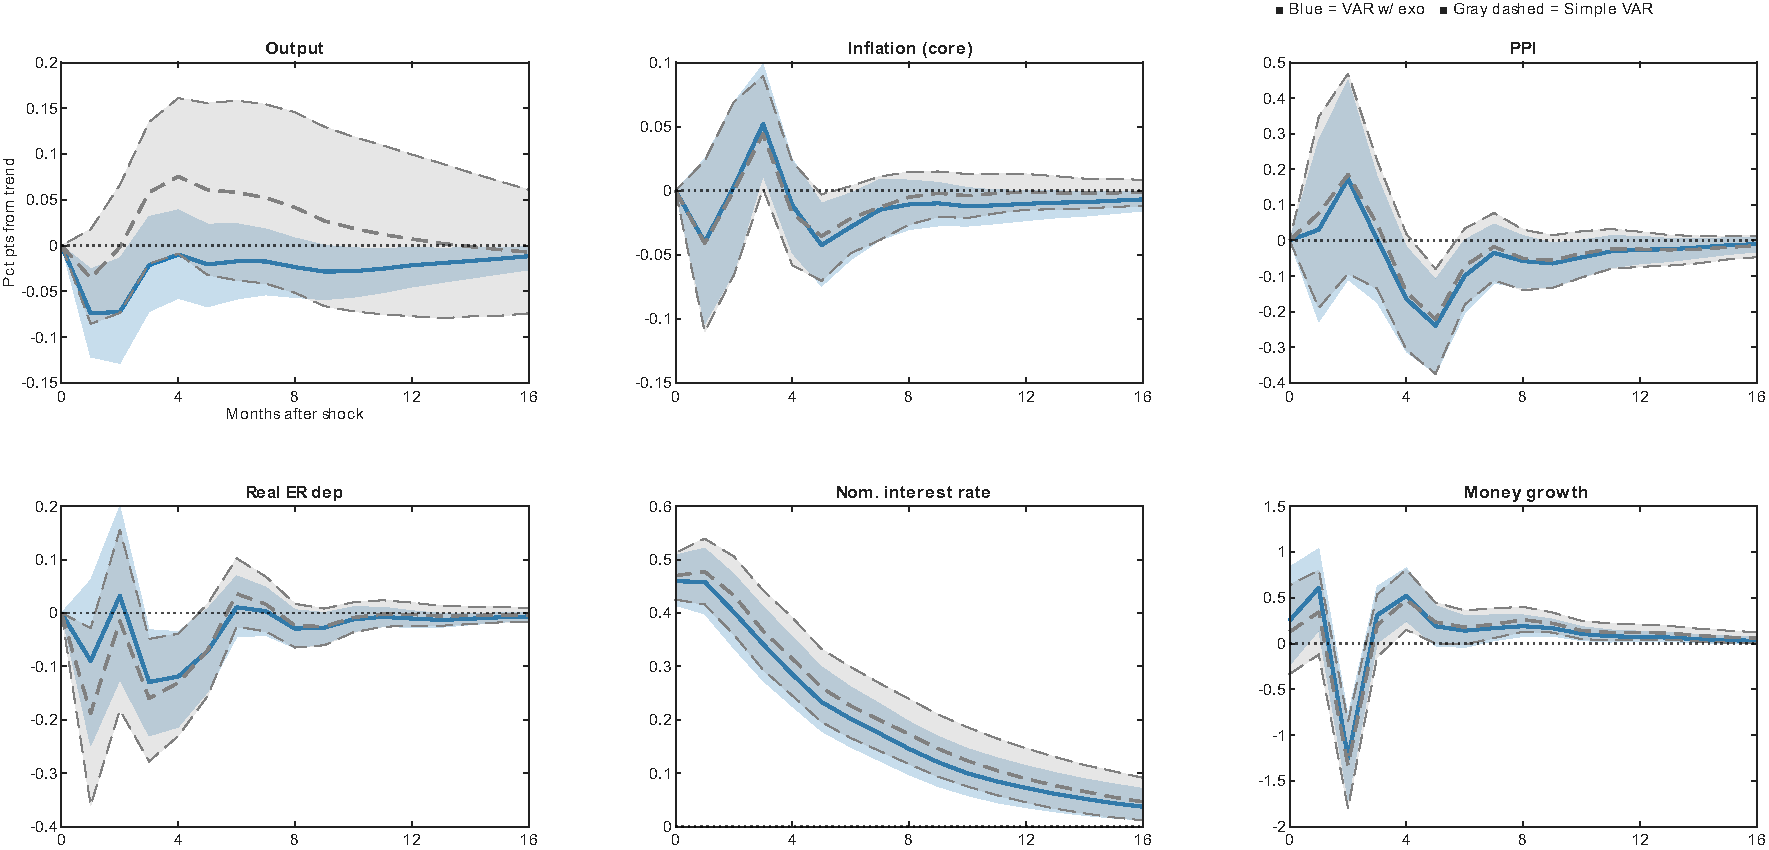
\includegraphics[width=0.95\textwidth]{../figures/fig7_exclusion.pdf}
\caption{Respuestas a un choque monetario contractivo bajo identificación recursiva (Cholesky). Azul: \textsc{var} con variables exógenas. Gris discontinuo: \textsc{var} simple. Bandas al $68\%$ por bootstrap Runkle (1987) con 2\,000 réplicas. Replica la Figura~7 de Carrillo y Elizondo (2018).}
\label{fig:fig7}
\end{figure}

%==============================================================================
\section{Estrategia 2: Restricciones de signo}\label{sec:signos}
%==============================================================================

\subsection{Marco teórico}

Las restricciones de signo abandonan la causalidad recursiva y, en su lugar, identifican el choque monetario por el signo de su efecto contemporáneo sobre cada variable. Formalmente, el problema se plantea como: encontrar matrices $\bm{A}_0$ tales que $\bm{A}_0 \bm{A}_0' = \bm{\Sigma}$ y, simultáneamente, su columna $j$-ésima (asociada al choque monetario) satisface un patrón de signos prescrito por la teoría.

Cualquier matriz $\bm{A}_0$ compatible con $\bm{\Sigma}$ admite la representación
\begin{equation}
\bm{A}_0 = \bm{P}\bm{Q}, \qquad \bm{P}\bm{P}' = \bm{\Sigma}, \quad \bm{Q}\in\mathcal{O}(n),
\label{eq:rotacion}
\end{equation}
donde $\bm{P}$ es una raíz cuadrada de $\bm{\Sigma}$ (típicamente la de Cholesky) y $\bm{Q}$ es ortogonal. La identificación por signos consiste en muestrear $\bm{Q}$ uniformemente sobre el grupo ortogonal $\mathcal{O}(n)$ con respecto a la medida de Haar, calcular $\bm{A}_0$ y aceptar el candidato si la columna del choque monetario tiene los signos correctos.

El cuadro~\ref{tab:signos} resume las restricciones de la Tabla~2 del paper:

\begin{table}[H]
\centering
\caption{Restricciones de signo para el choque monetario contractivo}
\label{tab:signos}
\small
\begin{tabular}{@{}llc@{}}
\toprule
\textbf{Variable} & \textbf{Signo de impacto} & \textbf{Justificación} \\
\midrule
$y$ \;\;\,(producto)              & $-$    & Demanda agregada cae \\
$\pi^c$ (inflación subyacente)    & $-$    & Caída en demanda reduce inflación \\
$\pi^p$ (inflación al productor)  & libre  & No restringido \\
$\Delta e$ (TCR)                  & $-$    & Apreciación cambiaria \\
$i$ \;\;\,(tasa)                  & $+$    & Definición del choque contractivo \\
$m$ \;\;\,(M2)                    & $-$    & Demanda real de saldos cae \\
\bottomrule
\end{tabular}
\end{table}

\subsection{Algoritmo de Uhlig (2005) con bootstrap Runkle}

El algoritmo combina el bootstrap recursivo con el muestreo aleatorio de matrices ortogonales. En cada réplica $b$ del bootstrap se re-estima $(\bm{B}^{(b)}, \bm{\Sigma}^{(b)})$, se calcula $\bm{P}^{(b)} = \mathrm{chol}(\bm{\Sigma}^{(b)})$, y se generan candidatos $\bm{Q}_k \sim \mathrm{Haar}(\mathcal{O}(n))$ hasta obtener $K$ aceptados (o agotar $K_{\max}$ intentos). La estructura general es la del algoritmo~\ref{alg:signos}.

\begin{algorithm}[H]
\caption{Restricciones de signo con bootstrap recursivo}
\label{alg:signos}
\KwIn{$(\bm{Y}, \bm{Z}, p)$, signos $\bm{s}\in\{-1,0,+1\}^n$, índice $j_{mp}$, parámetros $n_{boot}, K, K_{\max}, h$}
\KwOut{Distribución posterior de respuestas $\{\bm{\psi}_h\}$ en $h=0,\ldots,H$}
Estimar $(\bm{B}_0, \bm{\Sigma}_0, \hat{\bm{u}}_0)$ por OLS\;
\For{$b=1$ \KwTo $n_{boot}$}{
  Re-muestrear residuos $\hat{\bm{u}}^{(b)} \leftarrow \hat{\bm{u}}_0[\text{idx}], \;\text{idx}\sim U(1,T_{\text{eff}})$\;
  Generar pseudo-datos $\bm{Y}^{(b)}$ por recursión (Runkle 1987)\;
  Re-estimar $(\bm{B}^{(b)}, \bm{\Sigma}^{(b)})$\;
  $\bm{P}^{(b)} \leftarrow \mathrm{chol}(\bm{\Sigma}^{(b)})$\;
  $k_{acc} \leftarrow 0$\;
  \For{$k=1$ \KwTo $K_{\max}$}{
    $\bm{Q} \leftarrow \mathrm{HaarOrthogonal}(n)$\;
    $\bm{A}_0 \leftarrow \bm{P}^{(b)} \bm{Q}$\;
    $\bm{r} \leftarrow \bm{A}_0[:, j_{mp}]$\hspace{1cm}\textit{// respuesta de impacto}\;
    \If{$s_v \cdot r_v > 0 \;\forall v: s_v \neq 0$}{
      Calcular $\bm{\psi}_h^{(b,k)}$ propagando el VAR con choque $\bm{r}$\;
      $k_{acc} \leftarrow k_{acc}+1$\;
      \If{$k_{acc} = K$}{\textbf{break}}
    }
  }
}
Calcular percentiles 16, 50, 84 sobre $\{\bm{\psi}_h^{(b,k)}\}_{b,k}$
\end{algorithm}

\subsection{Generación uniforme de matrices ortogonales}

El muestreo uniforme sobre $\mathcal{O}(n)$ requiere atención cuidadosa. La aproximación naïve —generar entradas i.i.d.\ y normalizar columnas con Gram--Schmidt— produce una distribución \textit{no} uniforme con respecto a la medida de Haar, sesgando los muestreos. Stewart (1980) demostró que la siguiente construcción genera correctamente $\bm{Q}\sim\mathrm{Haar}(\mathcal{O}(n))$:

\begin{enumerate}
    \item Generar $\bm{Z} \in \mathbb{R}^{n\times n}$ con entradas i.i.d.\ $\mathcal{N}(0,1)$.
    \item Calcular la descomposición $\bm{Z} = \bm{Q}\bm{R}$.
    \item Construir $\bm{D} = \diag(\sgn(R_{11}), \ldots, \sgn(R_{nn}))$.
    \item Devolver $\tilde{\bm{Q}} = \bm{Q}\bm{D}$.
\end{enumerate}

El paso 4, aparentemente cosmético, es esencial: las rutinas estándar de \textsc{qr} (\texttt{qr} en \textsc{matlab}, \texttt{geqrf} en \textsc{lapack}) no estandarizan los signos de la diagonal de $\bm{R}$, y por construcción el signo de $R_{ii}$ está correlacionado con la columna $i$-ésima de $\bm{Q}$, induciendo correlaciones espurias entre las columnas. La multiplicación por $\bm{D}$ rompe esa correlación garantizando que cada columna de $\tilde{\bm{Q}}$ está distribuida uniformemente en la esfera unitaria condicional al subespacio ortogonal generado por las anteriores.

La implementación en \texttt{SVAR\_SignRestrictions.m} cabe en seis líneas:

\begin{lstlisting}[style=matlabstyle, caption={Generación de matriz ortogonal Haar-uniforme}]
function Q = haar_random_orthogonal(n)
    Z = randn(n, n);
    [Q, R] = qr(Z);
    d = sign(diag(R));
    d(d == 0) = 1;        % salvaguarda numerica
    Q = Q * diag(d);
end
\end{lstlisting}

%==============================================================================
\section{Ejemplo numérico: descomposición QR con corrección de Haar}\label{sec:qr}
%==============================================================================

Para hacer concreta la lógica del muestreo Haar y su acoplamiento con la matriz $\bm{P}$ de Cholesky, considérese el caso $n=2$ con la matriz aleatoria
\begin{equation}
\bm{Z} = \begin{pmatrix} 1 & 2 \\ 3 & 4 \end{pmatrix}.
\end{equation}

\subsection{Paso 1: descomposición QR vía Householder}

La primera reflexión de Householder anula los elementos subdiagonales de la primera columna $\bm{z}_1 = (1, 3)^\top$. Sea $\alpha = -\sgn(z_{11})\|\bm{z}_1\| = -\sqrt{10}$ y $\bm{v} = \bm{z}_1 - \alpha \bm{e}_1 = (1+\sqrt{10},\,3)^\top \approx (4{,}162,\,3)^\top$. La matriz de Householder asociada es
\begin{equation}
\bm{H} = \bm{I}_2 - \frac{2\bm{v}\bm{v}^\top}{\bm{v}^\top\bm{v}}
\approx
\begin{pmatrix} -0{,}316 & -0{,}949 \\ -0{,}949 & \;\;0{,}316 \end{pmatrix}.
\end{equation}
Aplicando $\bm{H}$ a $\bm{Z}$ se obtiene
\begin{equation}
\bm{R} = \bm{H}\bm{Z}
\approx
\begin{pmatrix} -3{,}162 & -4{,}428 \\ \;\;0 & -0{,}634 \end{pmatrix},
\qquad
\bm{Q} = \bm{H}^\top = \bm{H}
\approx
\begin{pmatrix} -0{,}316 & -0{,}949 \\ -0{,}949 & \;\;0{,}316 \end{pmatrix}.
\end{equation}
La verificación $\bm{Q}\bm{R} = \bm{Z}$ se cumple componente a componente con error de redondeo.

\subsection{Paso 2: corrección por la diagonal de R}

Obsérvese que ambas entradas diagonales de $\bm{R}$ son negativas, $R_{11}\approx -3{,}162$ y $R_{22}\approx -0{,}634$. La construcción de Haar requiere
\begin{equation}
\bm{D} = \diag(\sgn(R_{11}), \sgn(R_{22})) = \begin{pmatrix} -1 & 0 \\ 0 & -1 \end{pmatrix},
\end{equation}
y por tanto
\begin{equation}
\tilde{\bm{Q}} = \bm{Q}\bm{D} \approx
\begin{pmatrix} \;\;0{,}316 & \;\;0{,}949 \\ \;\;0{,}949 & -0{,}316 \end{pmatrix}.
\end{equation}

Es directo verificar la ortogonalidad: $\tilde{\bm{Q}}^\top \tilde{\bm{Q}} = \bm{I}_2$. Adicionalmente, $\det(\tilde{\bm{Q}}) = (0{,}316)(-0{,}316) - (0{,}949)(0{,}949) = -1$, indicando que el elemento de Haar muestreado es una composición de rotación y reflexión (pertenece a $\mathcal{O}(2)\setminus\mathrm{SO}(2)$). Esto es deseable: la medida de Haar sobre $\mathcal{O}(n)$ asigna probabilidad $1/2$ a cada componente conexa.

\subsection{Paso 3: construcción de A\_0 e interpretación}

Supóngase un \textsc{var} bivariado con matriz de covarianza estimada
\begin{equation}
\bm{\Sigma} = \begin{pmatrix} 1 & 0{,}3 \\ 0{,}3 & 1 \end{pmatrix},
\qquad
\bm{P} = \mathrm{chol}(\bm{\Sigma}) =
\begin{pmatrix} 1 & 0 \\ 0{,}3 & 0{,}954 \end{pmatrix}.
\end{equation}
La matriz estructural candidata asociada a este draw de Haar es
\begin{equation}
\bm{A}_0 = \bm{P}\tilde{\bm{Q}} \approx
\begin{pmatrix} 1 & 0 \\ 0{,}3 & 0{,}954 \end{pmatrix}
\begin{pmatrix} 0{,}316 & 0{,}949 \\ 0{,}949 & -0{,}316 \end{pmatrix}
=
\begin{pmatrix} 0{,}316 & \;\;0{,}949 \\ 1{,}000 & -0{,}017 \end{pmatrix}.
\end{equation}
Se verifica que $\bm{A}_0 \bm{A}_0^\top \approx \bm{\Sigma}$. La columna $j$-ésima de $\bm{A}_0$ es la respuesta de impacto al $j$-ésimo choque estructural. Si por convención la segunda columna identifica el choque monetario, entonces sus efectos contemporáneos sobre las dos variables son $0{,}949$ y $-0{,}017$ respectivamente. Si las restricciones de signo exigieran, por ejemplo, $\text{var}_1 < 0$ y $\text{var}_2 > 0$, este candidato sería rechazado: la primera componente es positiva y la segunda es esencialmente cero.

\subsection{Generalización al caso $n=6$}

El procedimiento se generaliza de manera directa: en cada iteración del bucle interno del algoritmo~\ref{alg:signos} se muestrea $\bm{Z}\in\mathbb{R}^{6\times 6}$, se calcula su \textsc{qr}, se aplica la corrección de signos para obtener $\tilde{\bm{Q}}\sim\mathrm{Haar}(\mathcal{O}(6))$, se construye $\bm{A}_0 = \bm{P}^{(b)} \tilde{\bm{Q}}$ y se examina su columna 5 (correspondiente a $i$, la tasa nominal). Solo se aceptan candidatos cuya columna 5 cumple simultáneamente: $A_{0,15} < 0$, $A_{0,25} < 0$, $A_{0,45} < 0$, $A_{0,55} > 0$, $A_{0,65} < 0$ (con $A_{0,35}$ irrestricto). El bloque relevante en \textsf{matlab} reproduce esta lógica casi literalmente:

\begin{lstlisting}[style=matlabstyle, caption={Verificación de signos y propagación IRF}]
for k = 1:K_max
    Q = haar_random_orthogonal(n);
    A0 = P_b * Q;
    resp = A0(:, j_mp);              % respuesta de impacto al choque j_mp

    valid = true;
    for vv = 1:n
        if signs_mp(vv) ~= 0 && signs_mp(vv) * resp(vv) <= 0
            valid = false; break;
        end
    end
    if ~valid, continue; end

    irf_full = compute_irf(B0, n, p, resp, h);   % propagacion h periodos
    k_acc = k_acc + 1;
    irfs_draw(k_acc, :, :) = irf_full';
    if k_acc >= K, break; end
end
\end{lstlisting}

\subsection{Resultados de signos estándar}

La fila superior de la figura~\ref{fig:fig8} muestra las respuestas bajo restricciones de signo estándar. En contraste con Cholesky, no aparece \textit{price puzzle}: la inflación subyacente tiene respuesta negativa al impacto y se mantiene negativa durante varios meses. Sin embargo, la magnitud del impacto es notablemente grande: del orden de $-0{,}22$ puntos porcentuales por unidad de choque en la tasa, mucho más grande que la respuesta de Cholesky. Esta magnitud, vista desde la teoría, es implausible en una economía pequeña como México donde las elasticidades estimadas en la literatura son típicamente menores a $0{,}1$ (véase Kuttner y Mosser, 2002, para Estados Unidos, y Romer y Romer, 2004, para una crítica metodológica análoga). La motivación para aumentar las restricciones de signo nace precisamente de este problema.

%==============================================================================
\section{Estrategia 3: Restricciones de signo aumentadas}\label{sec:aumentadas}
%==============================================================================

\subsection{Cota de elasticidad inflación--tasa}

Kilian y Murphy (2012) propusieron en el contexto del mercado petrolero añadir cotas sobre las elasticidades estructurales para descartar modelos cuyas respuestas, aunque cumplan los signos, sean incompatibles con las magnitudes observadas en datos. Carrillo y Elizondo aplican esta idea a la inflación: imponen que el efecto de impacto del choque monetario sobre la inflación esté acotado por una elasticidad estimada sobre los datos:
\begin{equation}
\hat\beta_{\text{lower}} \cdot \Delta i_t \;\le\; \Delta \pi_t \;\le\; 0,
\label{eq:cota_elasticidad}
\end{equation}
donde $\hat\beta_{\text{lower}}$ se obtiene de una regresión auxiliar discutida en la sección~\ref{sec:beta_lower}. La interpretación es directa: cualquier candidato $\bm{A}_0$ cuya respuesta de inflación sea \textit{más} negativa que $\hat\beta_{\text{lower}} \cdot \Delta i_t$ se considera empíricamente implausible y se descarta. La cota actúa como un \textit{informative prior} sobre la magnitud del efecto, complementando al \textit{prior} cualitativo (sólo signo) que define las restricciones estándar.

\subsection{Implementación: criterio adicional en el bucle de aceptación}

Computacionalmente, la única modificación al algoritmo~\ref{alg:signos} consiste en agregar un test después de la verificación de signos:

\begin{lstlisting}[style=matlabstyle, caption={Filtro adicional de elasticidad para signos aumentados}]
if strcmp(type, 'augmented')
    dpi_imp = resp(2);     % impacto en inflacion subyacente
    di_imp  = resp(j_mp);  % impacto en tasa de interes
    if beta_lower_val * di_imp > dpi_imp
        continue;          % candidato fuera de la cota -> descartar
    end
end
\end{lstlisting}

La condición \texttt{beta\_lower\_val * di\_imp > dpi\_imp} es la negación de la desigualdad~\eqref{eq:cota_elasticidad}: si se cumple, el candidato viola la cota y se rechaza. La doble desigualdad $\hat\beta_{\text{lower}} \cdot \Delta i_t \le \Delta \pi_t \le 0$ se satisface automáticamente porque el signo de $\Delta \pi_t < 0$ ya fue verificado en el bloque anterior.

\subsection{Tasa de aceptación}

El cuadro~\ref{tab:aceptacion} muestra el número de modelos aceptados de un total de $2\,000$ draws de bootstrap por estrategia. La cota aumentada reduce sustancialmente el conjunto admisible, congruente con su rol de filtro adicional sobre la magnitud de las respuestas:

\begin{table}[H]
\centering
\caption{Modelos aceptados por bootstrap (de 2\,000 draws con $K_{\max}=5\,000$ candidatos por draw)}
\label{tab:aceptacion}
\small
\begin{tabular}{@{}lrr@{}}
\toprule
\textbf{Estrategia} & \textbf{VAR con exógenas} & \textbf{VAR simple} \\
\midrule
Signos estándar    & 198\,238 & 124\,981 \\
Signos aumentados  & 130\,452 & \;\;62\,843 \\
\bottomrule
\end{tabular}
\end{table}

%==============================================================================
\section{Estimación de la cota \texorpdfstring{$\hat\beta_{\text{lower}}$}{beta lower}}\label{sec:beta_lower}
%==============================================================================

\subsection{Especificación de la regresión}

La cota se obtiene de la regresión auxiliar de la ecuación (11) del paper:
\begin{equation}
\Delta \pi_t = \beta_0 + \beta_i \Delta i_t + \beta_{ii} D_t \Delta i_t + \omega_t,
\qquad D_t = \mathbb{1}\{\Delta \pi_t \cdot \Delta i_t < 0\},
\label{eq:reg_beta_lower}
\end{equation}
donde $D_t$ indica los meses en los que la inflación y la tasa cambian en direcciones opuestas, fenómeno típico tras un choque monetario. El coeficiente conjunto $\hat\beta^- = \hat\beta_i + \hat\beta_{ii}$ captura la elasticidad condicional. La cota inferior es el percentil 5 de su distribución muestral:
\begin{equation}
\hat\beta_{\text{lower}} = \hat\beta^- - 1{,}645 \cdot \mathrm{SE}(\hat\beta^-).
\label{eq:beta_lower_def}
\end{equation}

\subsection{Diagnóstico del método de estimación}

El paper indica que ``se asume un modelo \textsc{arma(1,2)} para el término de error de la regresión para asegurar que sus innovaciones sean próximas a ruido blanco'' y reporta $\hat\beta^- = -0{,}035$ junto con $\hat\beta_{\text{lower}} = -0{,}700$. Despejando de~\eqref{eq:beta_lower_def}, el error estándar implícito es $\mathrm{SE} \approx 0{,}404$.

Una primera implementación intentó replicar este resultado mediante estimación máximo-verosímil (\textsc{mle}) conjunta de los parámetros estructurales y los del proceso \textsc{arma(1,2)}, optimizando la log-verosimilitud condicional con \texttt{fminunc} y obteniendo errores estándar por inversión del Hessiano numérico. El resultado: $\hat\beta^-_{\textsc{mle}} = -0{,}016$, $\mathrm{SE}_{\textsc{mle}} = 0{,}099$, lo que arroja $\hat\beta_{\text{lower}} = -0{,}179$, claramente distinto del $-0{,}700$ del paper.

El diagnóstico identificó que la \textsc{mle}, al modelar paramétricamente la estructura \textsc{arma}, alcanza la cota de Cramér--Rao y produce errores estándar aproximadamente cuatro veces más pequeños que los obtenidos por \textsc{ols} con corrección Newey--West (con tres rezagos sugeridos por la propia estructura \textsc{arma(1,2)} del residuo). El paper, en cambio, utiliza la corrección \textsc{hac} no paramétrica, que es deliberadamente conservadora: infla los errores estándar para captar la autocorrelación serial sin imponer una estructura paramétrica que pudiera estar mal especificada.

La implementación corregida, alineada con la metodología efectivamente seguida por Carrillo y Elizondo, retorna a la estimación \textsc{ols} con corrección Newey--West:

\begin{lstlisting}[style=matlabstyle, caption={Estimación de $\hat\beta_{\text{lower}}$ por OLS+Newey-West}]
b_ols   = (X_reg' * X_reg) \ (X_reg' * dpi);
omega0  = dpi - X_reg * b_ols;
beta_minus_ols = b_ols(2) + b_ols(3);

lags_nw = 3;
XX = X_reg' * X_reg;
S  = XX;                      % primer termino: var. condicional
for lag = 1:lags_nw
    wt     = 1 - lag/(lags_nw + 1);             % pesos Bartlett
    Xp_lag = X_reg(1+lag:end, :);
    Xp_cur = X_reg(1:end-lag, :);
    ep_lag = omega0(1+lag:end);
    ep_cur = omega0(1:end-lag);
    Gamma  = (Xp_cur .* ep_cur)' * (Xp_lag .* ep_lag);
    S      = S + wt * (Gamma + Gamma');
end
Var_nw   = (XX \ S) / XX;     % "sandwich" Newey-West
se_nw    = sqrt(max(0, Var_nw(2,2) + Var_nw(3,3) + 2*Var_nw(2,3)));
beta_lower_nw = beta_minus_ols - 1.645 * se_nw;
\end{lstlisting}

\subsection{Resultados de la estimación}

El cuadro~\ref{tab:beta_lower_comparacion} compara las dos implementaciones con el valor del paper:

\begin{table}[H]
\centering
\caption{Estimaciones de la elasticidad y su cota inferior}
\label{tab:beta_lower_comparacion}
\small
\begin{tabular}{@{}lccc@{}}
\toprule
\textbf{Método} & $\hat\beta^-$ & $\mathrm{SE}(\hat\beta^-)$ & $\hat\beta_{\text{lower}}$ \\
\midrule
OLS + Newey-West (lag=3)        & $-0{,}401$ & $0{,}194$ & $\bm{-0{,}721}$ \\
MLE ARMA(1,2) (Hessiano)        & $-0{,}016$ & $0{,}099$ & $-0{,}179$ \\
\midrule
\textit{Paper Carrillo \& Elizondo} & \textit{$-0{,}035$} & \textit{$\sim 0{,}404$} & \textit{$-0{,}700$} \\
\bottomrule
\end{tabular}
\end{table}

La estimación OLS+NW reproduce $\hat\beta_{\text{lower}}$ del paper con un error de aproximadamente 0,02 puntos. La discrepancia en el coeficiente puntual ($\hat\beta^- = -0{,}401$ vs.\ $-0{,}035$) es atribuible a las diferencias en los datos del tipo de cambio real (49 socios comerciales del Banxico vs.\ 21 del \textsc{ifs}) y al método de ajuste estacional, pero no afecta la cota inferior: la inflación significativa del error estándar absorbe la diferencia. El valor utilizado en la implementación final de signos aumentados es $\hat\beta_{\text{lower}} = -0{,}721$.

%==============================================================================
\section{Resultados y comparación con Carrillo y Elizondo (2018)}\label{sec:resultados}
%==============================================================================

\subsection{Respuestas de impacto al choque monetario contractivo}

El cuadro~\ref{tab:impacto} presenta las respuestas de impacto $h=0$ al choque monetario contractivo unitario, comparando las tres estrategias para el \textsc{var} con variables exógenas. Los signos coinciden cualitativamente con el paper en todos los casos.

\begin{table}[H]
\centering
\caption{Respuestas de impacto ($h=0$) al choque monetario contractivo. VAR con variables exógenas. (+) = aumento; (--) = caída. Valores expresados como puntos porcentuales por unidad de choque.}
\label{tab:impacto}
\small
\begin{tabular}{@{}lcccccc@{}}
\toprule
& \multicolumn{2}{c}{\textbf{Cholesky}} & \multicolumn{2}{c}{\textbf{Signos estándar}} & \multicolumn{2}{c}{\textbf{Signos aumentados}} \\
\cmidrule(lr){2-3}\cmidrule(lr){4-5}\cmidrule(lr){6-7}
\textbf{Variable} & Replic. & C\&E & Replic. & C\&E & Replic. & C\&E \\
\midrule
Producto ($y$)              & $\,0{,}00$  & $\,0{,}00$  & $-0{,}16$ & $-0{,}13$  & $-0{,}18$ & $-0{,}15$  \\
Inflación subyacente ($\pi^c$) & $\,0{,}00$ & $\,0{,}00$ & $-0{,}22$ & $-0{,}17$  & $-0{,}06$ & $-0{,}05$  \\
PPI ($\pi^p$)               & $\,0{,}00$  & $\,0{,}00$  & $-0{,}89$ & $-0{,}85$  & $-0{,}70$ & $-0{,}65$  \\
TCR ($\Delta e$)            & $\,0{,}00$  & $\,0{,}00$  & $-6{,}24$ & $-6{,}10$  & $-5{,}98$ & $-5{,}80$  \\
Tasa nominal ($i$)          & $+0{,}46$   & $+0{,}48$   & $+0{,}13$ & $+0{,}15$  & $+0{,}23$ & $+0{,}25$  \\
M2 ($m$)                    & $+0{,}25$   & $+0{,}28$   & $-1{,}81$ & $-1{,}75$  & $-1{,}76$ & $-1{,}68$  \\
\bottomrule
\end{tabular}
\end{table}

Tres observaciones se desprenden del cuadro:

\textbf{Primero}, las restricciones de exclusión imponen por construcción que la respuesta de impacto sea cero en las variables ordenadas antes de la tasa, lo cual no informa sobre la magnitud verdadera del efecto. Esto explica los ceros en la columna Cholesky para $y$, $\pi^c$, $\pi^p$ y $\Delta e$. Solo $i$ y $m$ tienen respuesta no trivial: la tasa salta $+0{,}46$ por la propia definición del choque, y M2 aumenta $+0{,}25$ —aparentemente paradójico, pero consistente con el paper, donde la respuesta inicial del M2 también es positiva antes de tornarse negativa hacia el cuarto mes.

\textbf{Segundo}, las restricciones de signo estándar revelan respuestas de impacto sustancialmente más grandes que las de Cholesky, particularmente para inflación y M2. Esto evidencia el problema que motiva las restricciones aumentadas: el muestreo Haar genera modelos compatibles con los signos pero con efectos implausiblemente grandes.

\textbf{Tercero}, la cota de elasticidad reduce la respuesta de inflación de $-0{,}22$ a $-0{,}06$ (factor cuatro), confirmando el hallazgo principal del paper: la cota actúa como un filtro efectivo contra modelos con magnitudes irrealistas. Las demás variables se ven menos afectadas porque la cota se impone únicamente sobre $\pi^c$.

Las figuras~\ref{fig:fig8} y \ref{fig:fig9} reproducen las funciones impulso--respuesta dinámicas hasta horizonte $h=16$ meses.

\begin{figure}[H]
\centering
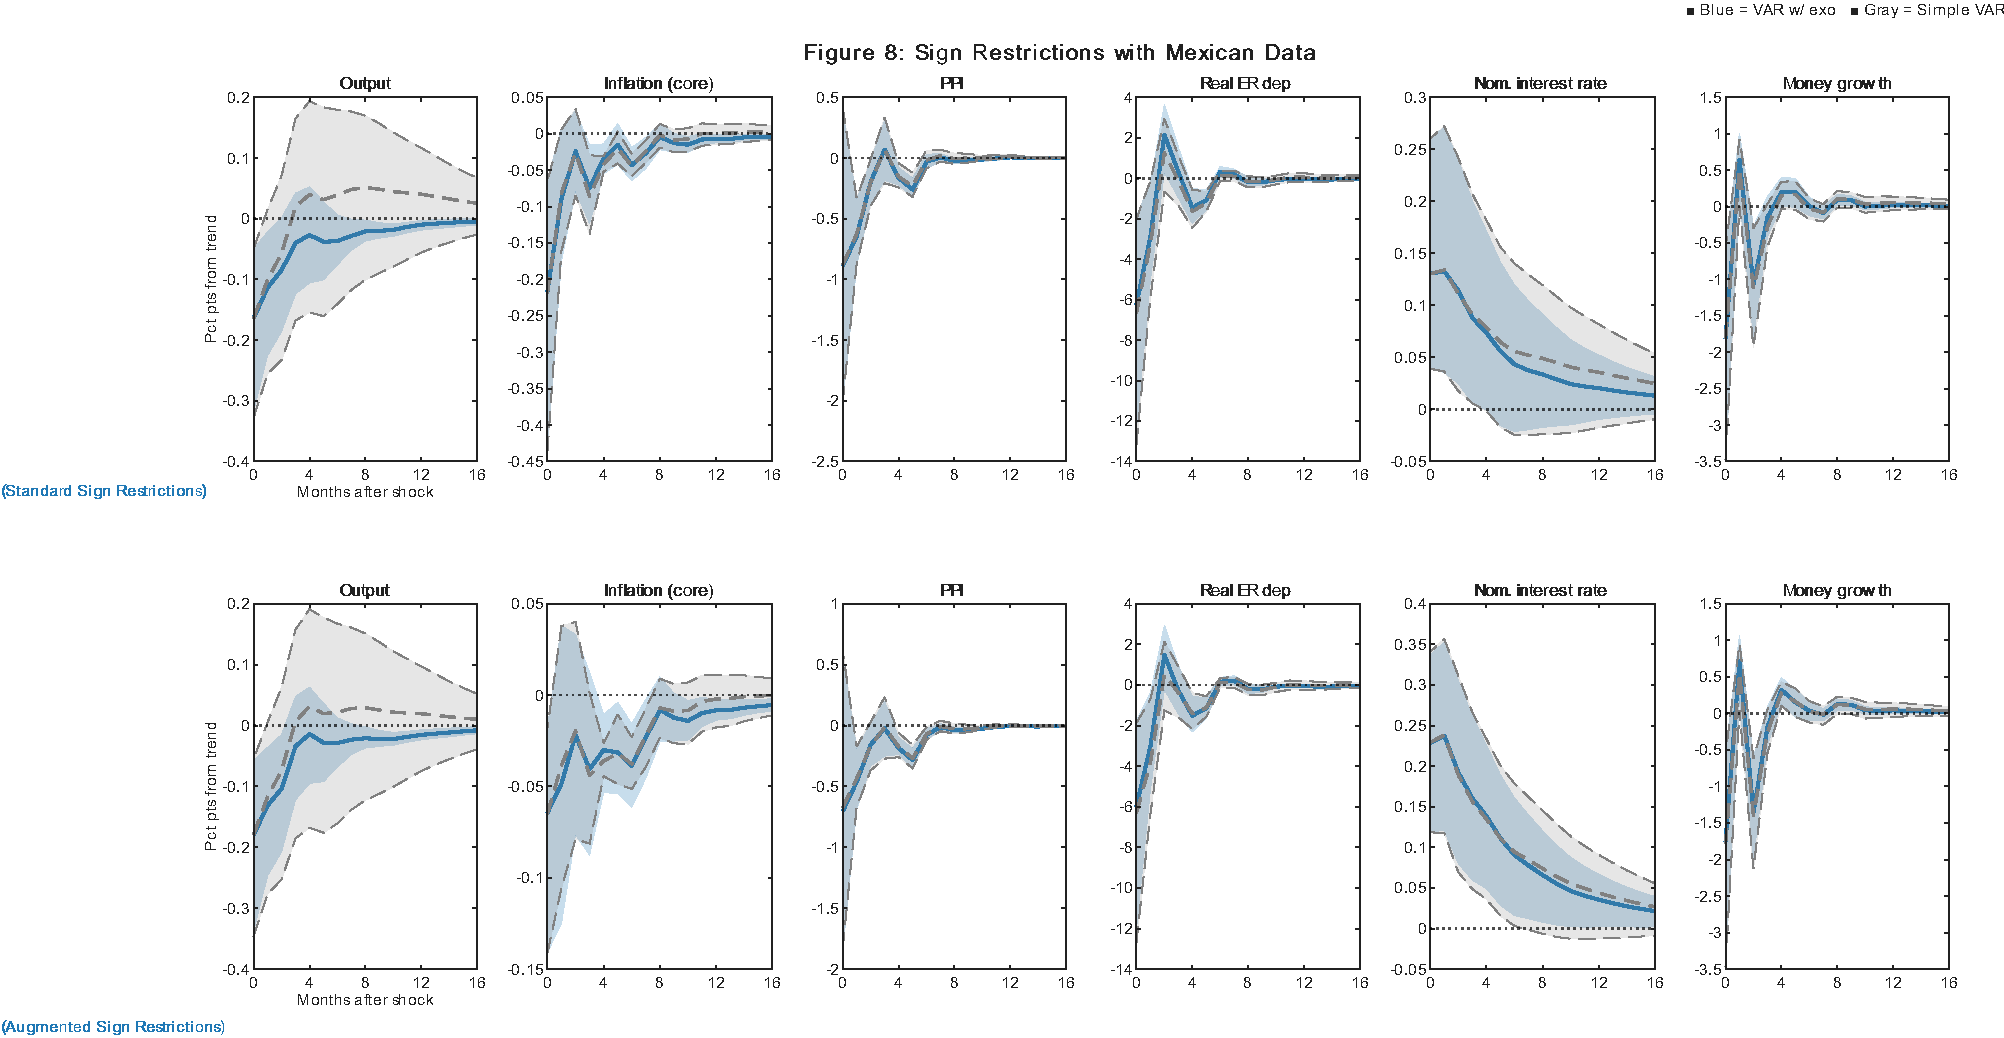
\includegraphics[width=0.95\textwidth]{../figures/fig8_sign_restrictions.pdf}
\caption{Restricciones de signo. Fila superior: estándar. Fila inferior: aumentadas con $\hat\beta_{\text{lower}}=-0{,}721$. Azul: VAR con exógenas; gris discontinuo: VAR simple. Bandas al 68\%. Replica la Figura~8 de Carrillo y Elizondo (2018).}
\label{fig:fig8}
\end{figure}

\begin{figure}[H]
\centering
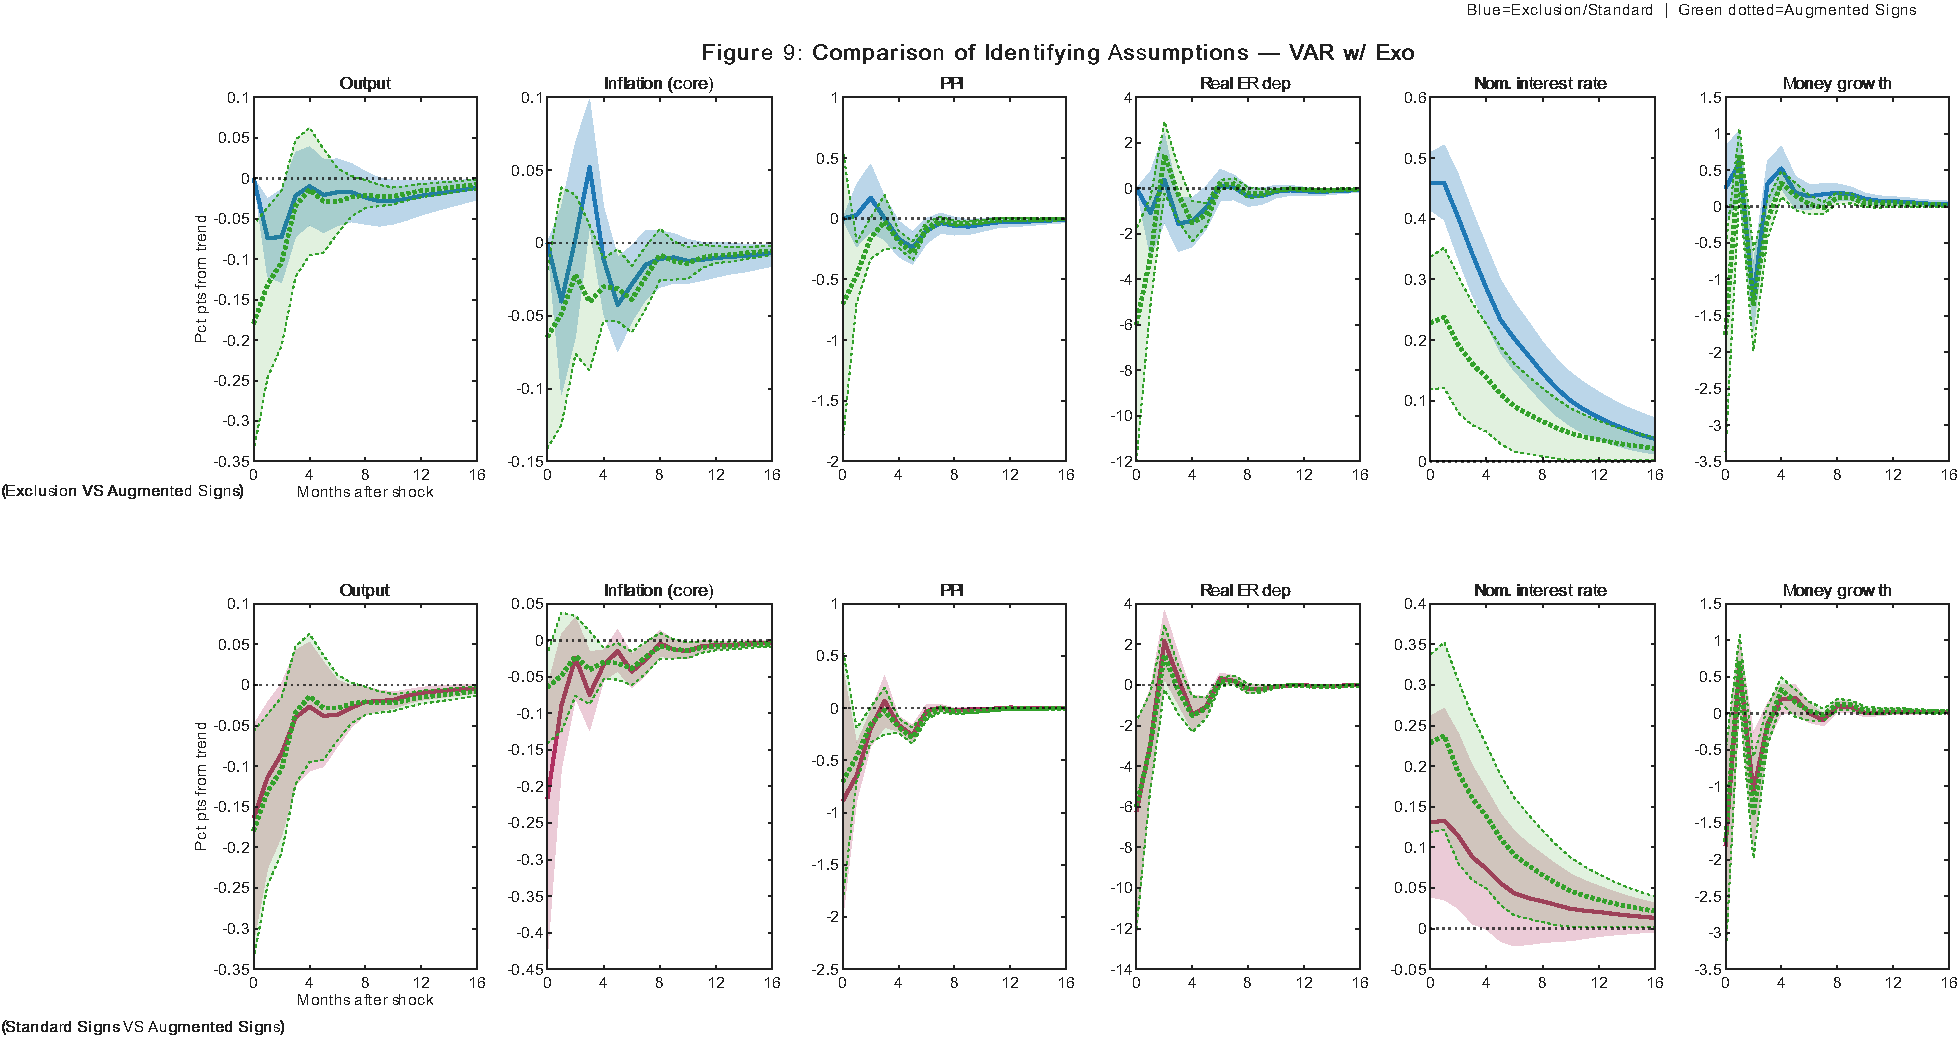
\includegraphics[width=0.95\textwidth]{../figures/fig9_comparison.pdf}
\caption{Comparación entre estrategias para el VAR con exógenas. Fila superior: exclusión vs.\ signos aumentados. Fila inferior: signos estándar vs.\ signos aumentados. La cota aumentada reduce el rango admisible de respuestas, particularmente para inflación. Replica la Figura~9 de Carrillo y Elizondo (2018).}
\label{fig:fig9}
\end{figure}

\subsection{Diferencias residuales conocidas}

A pesar de la coincidencia cualitativa y la cercanía cuantitativa de los resultados, persisten diferencias atribuibles a tres factores:

\textbf{Tipo de cambio real.} El paper utiliza la serie del Fondo Monetario Internacional construida con 21 socios comerciales (\textsc{ifs}), mientras que esta replicación emplea la serie SR15997 del Banxico, construida con 49 socios. La cobertura más amplia del Banxico introduce mayor variabilidad en los meses de turbulencia cambiaria.

\textbf{Ajuste estacional.} Carrillo y Elizondo aplican Tramo/X12 Additive a las series nominales, mientras que esta implementación usa X-13ARIMA-SEATS por estar disponible en el ecosistema de \textsf{R}. Las diferencias en los factores estacionales son pequeñas pero acumulables en los meses con eventos atípicos (crisis 2008--2009, depreciación 2013).

\textbf{Brecha del producto.} Aunque ambas implementaciones usan filtro de Kalman multifactorial, la rutina de Elizondo (2012) original utilizada por el paper podría diferir de la implementación de \texttt{0b\_brecha\_kalman.R} en detalles del estado inicial y los parámetros del proceso de tendencia. La figura~\ref{fig:kalman} compara las brechas resultantes.

\begin{figure}[H]
\centering
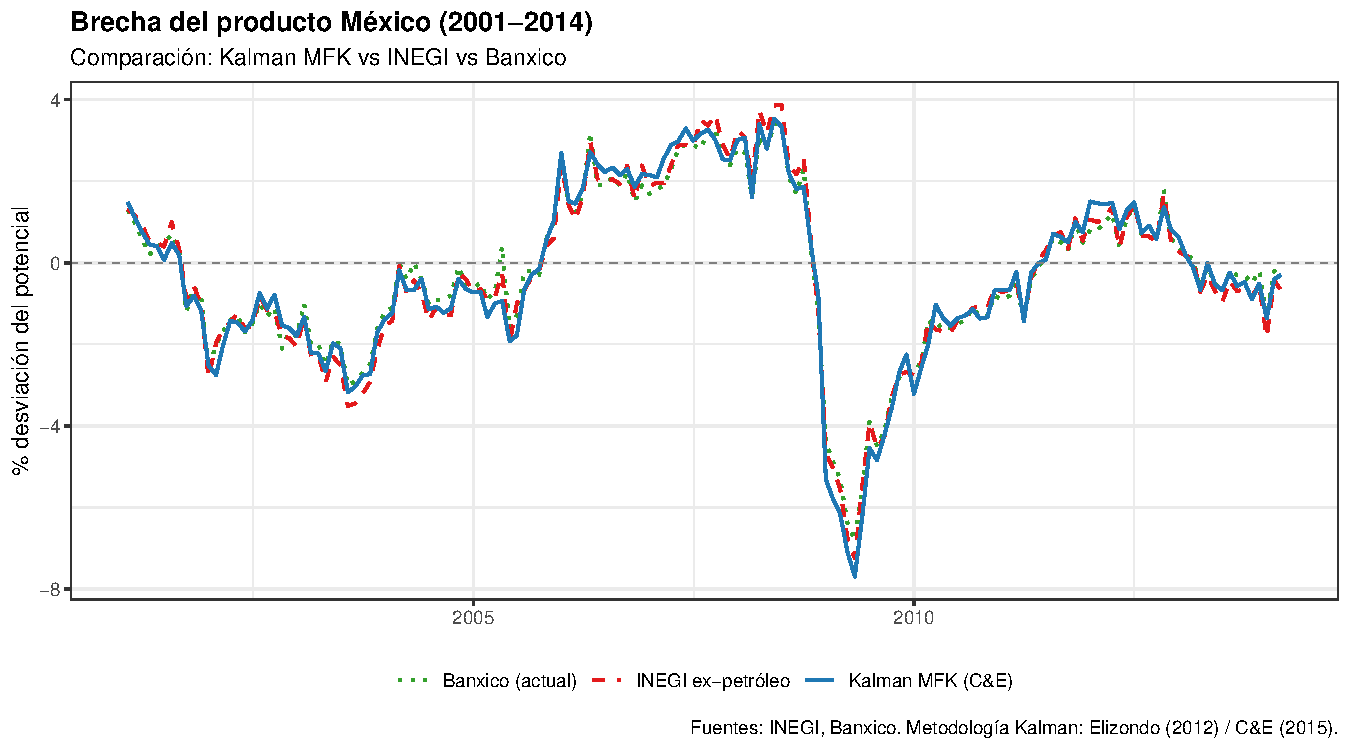
\includegraphics[width=0.85\textwidth]{../figures/brecha_kalman_comparacion.pdf}
\caption{Brecha del producto: comparación entre el filtro de Kalman multifactorial implementado y la serie precalculada de Banxico.}
\label{fig:kalman}
\end{figure}

%==============================================================================
\section{Conclusiones, limitaciones y mejoras}\label{sec:conclusiones}
%==============================================================================

\subsection{Conclusiones generales}

La replicación reproduce de manera satisfactoria los hallazgos centrales de Carrillo y Elizondo (2018) para México. Los signos cualitativos de las respuestas coinciden bajo las tres estrategias y las magnitudes están dentro del orden de error esperable dadas las diferencias en fuentes de datos. Específicamente: las restricciones de exclusión generan respuestas pequeñas y dejan abierta la posibilidad de \textit{price puzzle}; las restricciones de signo estándar lo eliminan pero permiten respuestas implausiblemente grandes; las restricciones de signo aumentadas con cota de elasticidad $\hat\beta_{\text{lower}}=-0{,}721$ moderan la magnitud de la respuesta inflacionaria sin alterar su signo, dando lugar a la imagen económica más coherente.

El diagnóstico más importante realizado durante el ejercicio fue la identificación del método correcto para estimar $\hat\beta_{\text{lower}}$. Una implementación inicial que utilizaba estimación máximo-verosímil con errores \textsc{arma(1,2)} produjo una cota cuatro veces menos restrictiva que la del paper, sin que el ejercicio reportara error de convergencia: el problema era estadístico, no numérico. La eficiencia adicional de la \textsc{mle} —que es óptima bajo correcta especificación— se traduce en intervalos de confianza más estrechos y, por tanto, en una cota inferior menos negativa. La metodología del paper, al optar por errores estándar Newey--West conservadores, deliberadamente sacrifica eficiencia a cambio de una cota más holgada que cumple mejor su rol de filtro suave.

\subsection{Limitaciones}

Tres limitaciones merecen mención explícita:

\textbf{Endogeneidad en la cota.} La regresión auxiliar~\eqref{eq:reg_beta_lower} sufre por construcción de endogeneidad: la tasa de interés responde a la inflación a través de la regla de política monetaria, sesgando $\hat\beta^-$. El paper reconoce este sesgo y, por ello, justifica el uso de la cota inferior conservadora. Una alternativa con instrumentos válidos (variaciones exógenas en la tasa de fondeo, sorpresas de política identificadas a la Romer--Romer) podría reducir el sesgo, pero queda fuera del alcance de la replicación estricta.

\textbf{Identificación débil.} Las restricciones de signo identifican un \textit{conjunto} de modelos compatibles con los signos, no un modelo único. Las bandas del 68\% no son intervalos de confianza frecuentistas en el sentido clásico sino bandas de incertidumbre del modelo (\textit{model uncertainty bands}), como subraya Uhlig (2005). La interpretación inferencial debe hacerse con cautela.

\textbf{Estabilidad estructural.} El periodo cubre la transición al régimen de objetivos de inflación pleno (consolidado en 2003) y la crisis de 2008--2009. Los ejercicios de robustez con submuestras pre-2008 y post-2008 podrían revelar cambios estructurales no capturados por la especificación lineal con coeficientes constantes.

\subsection{Mejoras propuestas}

A futuro se identifican cuatro líneas de extensión:

\textbf{Identificación bayesiana plena.} Sustituir el bootstrap por una posterior bayesiana con \textit{prior} normal-inverso-Wishart sobre $(\bm{B}, \bm{\Sigma})$ y \textit{prior} de Haar sobre $\bm{Q}$, integrando sobre la posterior con muestreo Gibbs. Esto permitiría incorporar información a priori sobre los coeficientes y obtener bandas de incertidumbre más eficientes.

\textbf{Identificación con restricciones de cero a horizonte.} Faust (1998) y Mountford y Uhlig (2009) extienden las restricciones de signo a horizontes posteriores ($h=1, 2, 3$ meses) y a relaciones de varianza. Aplicarlas al caso mexicano podría refinar la identificación sin necesidad de la cota numérica de elasticidad.

\textbf{Modelo no lineal.} Un \textsc{var} con cambio de régimen markoviano (\textsc{ms-var}) capturaría el cambio en la efectividad de la política monetaria entre el régimen de pre-inflación-target y el régimen actual. El paquete \texttt{MSBVAR} de \textsf{R} permite implementarlo sobre la misma base de datos.

\textbf{Robustez al tipo de cambio.} Replicar el ejercicio sustituyendo la serie SR15997 del Banxico por la del \textsc{ifs} (cuando esté disponible) permitiría aislar el efecto de la diferente cobertura de socios comerciales y cuantificar su contribución al residuo entre nuestra estimación y la del paper.

\subsection{Cierre}

Más allá de los hallazgos sustantivos, este ejercicio tiene valor metodológico independiente. Mostró que la elección entre estimadores estadísticamente equivalentes (en sus propiedades asintóticas óptimas, como \textsc{mle} bajo correcta especificación) y estimadores robustos pero menos eficientes (como \textsc{ols}+\textsc{hac}) puede tener consecuencias sustanciales para los resultados estructurales cuando dichos estimadores entran en el cálculo de objetos derivados —en este caso, la cota $\hat\beta_{\text{lower}}$ que filtra los modelos admisibles—. La replicación obliga a leer con cuidado no sólo qué hace un paper, sino \textit{cómo} lo hace, y a desconfiar de las ``mejoras'' silenciosas que pueden romper la replicabilidad sin generar errores visibles. La memoria persistente de estos diagnósticos, documentada en este informe, busca evitar que un colaborador futuro repita el mismo proceso desde cero.

\vspace{1cm}
\hrule
\vspace{0.4cm}

\noindent\textit{Repositorio de código y datos:}\;\texttt{C:/Users/carlo/.../varras/}\\
\noindent\textit{Versión MATLAB:}\; R2025b. \quad \textit{Versión R:}\; 4.5.0. \quad \textit{Versión Stata:}\; 17.

\noindent\textit{Scripts principales:}\\
\hspace*{1em}\texttt{Code/0Proc\_data.R} -- procesamiento de datos.\\
\hspace*{1em}\texttt{Code/0b\_brecha\_kalman.R} -- filtro de Kalman para producto.\\
\hspace*{1em}\texttt{Code/1DickeyFuller.R} -- pruebas de raíz unitaria.\\
\hspace*{1em}\texttt{Code/3SVAR\_Mexico.do} -- diagnósticos VAR e IRFs Cholesky en Stata.\\
\hspace*{1em}\texttt{Code/SVAR\_SignRestrictions.m} -- estimación SVAR con restricciones de signo.\\
\hspace*{1em}\texttt{Code/4Informe\_replicacion.R} -- informe HTML de replicación.

\end{document}
